\documentclass{article}
\usepackage{arxiv}

\usepackage[utf8]{inputenc}
\usepackage[english, russian]{babel}
\usepackage[T1]{fontenc}
\usepackage{url}
\usepackage{booktabs}
\usepackage{amsfonts}
\usepackage{nicefrac}
\usepackage{microtype}
\usepackage{lipsum}
\usepackage{graphicx}
\usepackage{natbib}
\usepackage{doi}



\title{Клеточные автоматы в задаче моделирования живых систем}

\author{ Cкороходов А.С. \\
	МГУ им. М.В. Ломоносова, \\
	кафедра математических методов \\ прогнозирования, 417 группа\\
	\texttt{s02200480@gse.cs.msu.ru} \\
	\And
	Гуров С.И. \\
	доцент, к. ф.-м. н.\\
	МГУ им. М.В. Ломоносова\\
	ф-т ВМК, кафедра ММП\\
	\texttt{sgur@cs.msu.ru } \\
	%% \AND
	%% Coauthor \\
	%% Affiliation \\
	%% Address \\
	%% \texttt{email} \\
	%% \And
	%% Coauthor \\
	%% Affiliation \\
	%% Address \\
	%% \texttt{email} \\
	%% \And
	%% Coauthor \\
	%% Affiliation \\
	%% Address \\
	%% \texttt{email} \\
}
\date{}

\renewcommand{\shorttitle}{\textit{arXiv} Template}

%%% Add PDF metadata to help others organize their library
%%% Once the PDF is generated, you can check the metadata with
%%% $ pdfinfo template.pdf
\hypersetup{
pdftitle={Клеточные автоматы в задаче моделирования живых систем},
pdfsubject={q-bio.NC, q-bio.QM},
pdfauthor={David S.~Hippocampus, Elias D.~Striatum},
pdfkeywords={First keyword, Second keyword, More},
}

\begin{document}
\maketitle

\begin{abstract}
	Клеточные автоматы (КлА) - это модели, которые генерируют крупномасштабный паттерн из мелкомасштабных локальных процессов. КлА используют сетчатую структуру в качестве поля для вычислений своих состояний. Последовательные состояния ячеек, расположенных на сетке, вычисляются в соответствии с набором правил. Переходы состояний зависят от состояния отдельных ячеек и состояния ячеек в локальной окрестности. Клеточные автоматы применяются в качестве подхода к моделированию во многих научных дисциплинах и используются в задаче моделирования живых процессов как один из наиболее популярных типов моделей для изучения пространственных процессов в динамике. В работе я обсуждаю основные области применения КлА в моделировании живых процессов с акцентом на градостроительное моделирование.
\end{abstract}


\keywords{Клеточные автоматы \and Моделирование живых систем}

\section{Введение}
	Клеточные автоматы (КлА) - это пространственно-временные дискретные системы, которые могут моделировать динамические сложные системы. На сегодняшний день известно множество проблемных областей, где были успешно применены КлА. 
	Различные клеточные автоматы могут демонстрировать весьма разнообразное поведение, которое может быть адаптировано для целей обработки информации за счет выбора (а) закона изменения состояния элемента и (б) конкретного определения понятия "ближайшие соседи".
	Клеточные автоматы (КлА) - один из наиболее распространенных методов, используемых для моделирования процесса урбанизации. Городские модели на основе КлА используют правила перехода для получения пространственных моделей роста городов и городской динамики с течением времени. 
	Город представляет собой типичную сложную систему, которая характеризуется свойством самоорганизации. Понимание процесса городского развития крайне важно при планировании городского развития и управлении устойчивым ростом. Процесс городского развития включает в себя множество действующих лиц, различные модели поведения и различную политику, что приводит к их пространственным и временным сложностям. Недавно разработанная технология клеточных автоматов (КлА) привлекает все больше внимания в GIS-моделировании благодаря своей простоте, прозрачности и  широким возможностям динамического пространственного моделирования.
	В этой работе будет совершена попытка в построении модели Клеточного Автомата симулирующего процесс развития города с ростом населения, вывод необходимых параметров, точно описывающих задачу.

\section{Постановка задачи}
\label{sec:headings}

\lipsum[4] See Section \ref{sec:headings}.

\subsection{Headings: second level}
\lipsum[5]
\begin{equation}
	\xi _{ij}(t)=P(x_{t}=i,x_{t+1}=j|y,v,w;\theta)= {\frac {\alpha _{i}(t)a^{w_t}_{ij}\beta _{j}(t+1)b^{v_{t+1}}_{j}(y_{t+1})}{\sum _{i=1}^{N} \sum _{j=1}^{N} \alpha _{i}(t)a^{w_t}_{ij}\beta _{j}(t+1)b^{v_{t+1}}_{j}(y_{t+1})}}
\end{equation}

\subsubsection{Headings: third level}
\lipsum[6]

\paragraph{Paragraph}
\lipsum[7]



\section{Examples of citations, figures, tables, references}
\label{sec:others}

\subsection{Citations}
Citations use \verb+natbib+. The documentation may be found at
\begin{center}
	\url{http://mirrors.ctan.org/macros/latex/contrib/natbib/natnotes.pdf}
\end{center}

Here is an example usage of the two main commands (\verb+citet+ and \verb+citep+): Some people thought a thing \citep{kour2014real, hadash2018estimate} but other people thought something else \citep{kour2014fast}. Many people have speculated that if we knew exactly why \citet{kour2014fast} thought this\dots

\subsection{Figures}
\lipsum[10]
See Figure \ref{fig:fig1}. Here is how you add footnotes. \footnote{Sample of the first footnote.}
\lipsum[11]

\begin{figure}
	\centering
	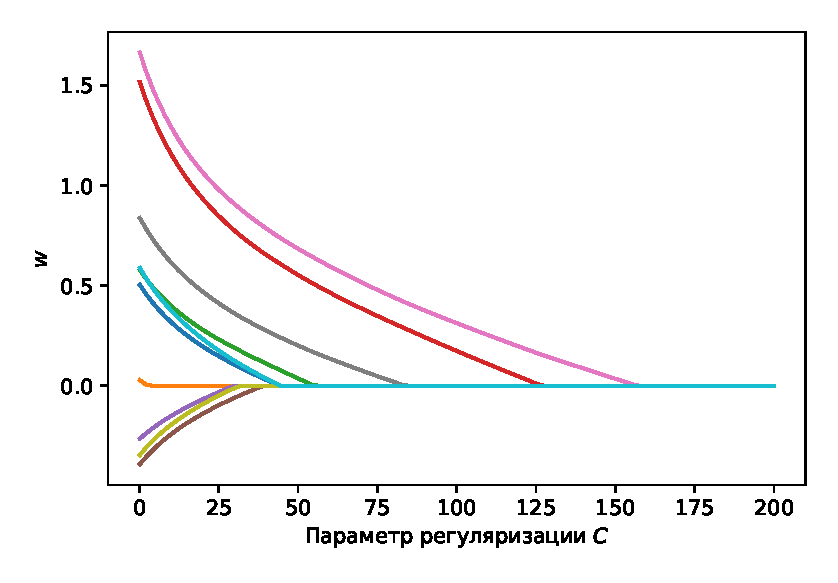
\includegraphics[width=0.5\textwidth]{../figures/log_reg_cs_exp.eps}
	\caption{Sample figure caption.}
	\label{fig:fig1}
\end{figure}

\subsection{Tables}
See awesome Table~\ref{tab:table}.

The documentation for \verb+booktabs+ (`Publication quality tables in LaTeX') is available from:
\begin{center}
	\url{https://www.ctan.org/pkg/booktabs}
\end{center}


\begin{table}
	\caption{Sample table title}
	\centering
	\begin{tabular}{lll}
		\toprule
		\multicolumn{2}{c}{Part}                   \\
		\cmidrule(r){1-2}
		Name     & Description     & Size ($\mu$m) \\
		\midrule
		Dendrite & Input terminal  & $\sim$100     \\
		Axon     & Output terminal & $\sim$10      \\
		Soma     & Cell body       & up to $10^6$  \\
		\bottomrule
	\end{tabular}
	\label{tab:table}
\end{table}

\subsection{Lists}
\begin{itemize}
	\item Lorem ipsum dolor sit amet
	\item consectetur adipiscing elit.
	\item Aliquam dignissim blandit est, in dictum tortor gravida eget. In ac rutrum magna.
\end{itemize}


\bibliographystyle{unsrtnat}
\bibliography{references}

\end{document}
